\documentclass[11pt, oneside]{article}
\usepackage{amsmath}
\usepackage{amssymb}
\usepackage[usenames,dvipsnames]{xcolor}
\usepackage{tikz}
\usepackage{xcolor}
\usetikzlibrary{snakes}
\usetikzlibrary{decorations}
\usetikzlibrary{trees}
\usetikzlibrary{decorations.pathmorphing}
\usetikzlibrary{decorations.markings}
\usetikzlibrary{external}
\usetikzlibrary{intersections}
\usetikzlibrary{shapes,arrows}
\usetikzlibrary{arrows.meta}
\usetikzlibrary{calc}
\usetikzlibrary{shapes.misc}
\usetikzlibrary{decorations.text}
\usetikzlibrary{backgrounds}
\usetikzlibrary{fadings}
\usepackage{tikz}
\usetikzlibrary{patterns}
\usetikzlibrary{positioning}
\usetikzlibrary{tikzmark,calc,arrows,shapes,decorations.pathreplacing}
\tikzset{
        cross/.style={cross out, draw=black, minimum size=2*(#1-\pgflinewidth), inner sep=0pt, outer sep=0pt},
	branchCut/.style={postaction={decorate},
		snake=zigzag,
		decoration = {snake=zigzag,segment length = 2mm, amplitude = 2mm}	
    }}

\begin{document}

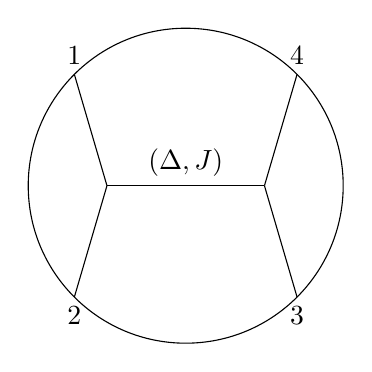
\begin{tikzpicture}
        % Circle boundary
        \draw (0,0) circle (2 cm);
        
        % Points
        \coordinate (1) at (-1.41421,1.41421);
        \coordinate (2) at (-1.41421,-1.41421);
        \coordinate (C) at (-1,0);
        \coordinate (D) at (1,0);
         \coordinate (4) at (1.41421,1.41421);
        \coordinate (3) at (1.41421,-1.41421);
              
        % Lines connecting points
        \draw (1) -- (C);
        \draw (2) -- (C);
        \draw (C) -- (D) node[midway, above] {\((\Delta,J)\)};
         \draw (3) -- (D);
        \draw (4) -- (D);
                  
        % Points
        \fill (1)  node[above] {$1$};
        \fill (2) node[below] {$2$};
        \fill (3) node[below] {$3$};
         \fill (4) node[above] {$4$};
       \end{tikzpicture}

\end{document}